%-------------------------
%device-revisited.tex
%(c) H.Buchmann FHNW 2018
%export TEXINPUTS=${HOME}/fhnw/edu/:${HOME}/fhnw/edu/tinL/config/latex:${HOME}/fhnw/edu/config//:
%-------------------------
\documentclass{beamer}
\usepackage{latex/beamer}
%---------------------
%local defines
%(c) H.Buchmann FHNW 2009
%$Id$
%---------------------
\newcommand{\target} {\beaglebone\xspace}
\newcommand{\targetS}{{\bf BBG}\xspace}
\newcommand{\host}   {{\em Host}\xspace}
\newcommand{\targetroot} {{\bf target-root}\xspace}
\newcommand{\kernel} {{\bf kernel}\xspace}
\renewcommand{\c}{{\bf C}\xspace}
\newcommand{\cpp}{{\bf C++}\xspace}
\newcommand{\posix}{{\bf POSIX}\xspace}

\input{/home/buchmann/latex/dirtree/dirtree.tex}
\usepackage{svg}
\usepackage[absolute]{textpos}
\setlength{\TPHorizModule}{1mm}
\setlength{\TPVertModule}{1mm}

\begin{document}


\newcommand{\ksp}{{\em kernel-space}\xspace}
\newcommand{\usp}{{\em user-space}\xspace}
\newcommand{\hw}{{\em HW}\xspace}
\title[Hardwarwe]{Hardware}

\frame{\titlepage}

\begin{frame}{Um was geht es ?}{Hardware}
 \begin{itemize}
  \item \usp $\to$ \ksp $\to$ \hw
  \begin{itemize}
   \item via  {\em sysfs}
  \end{itemize}
  \item \hw $\to$  \ksp $\to$ \usp
  \begin{itemize}
   \item Interrupts
  \end{itemize}  
 \end{itemize}
\end{frame}

\begin{frame}{Unsere Hardware}
\begin{center}
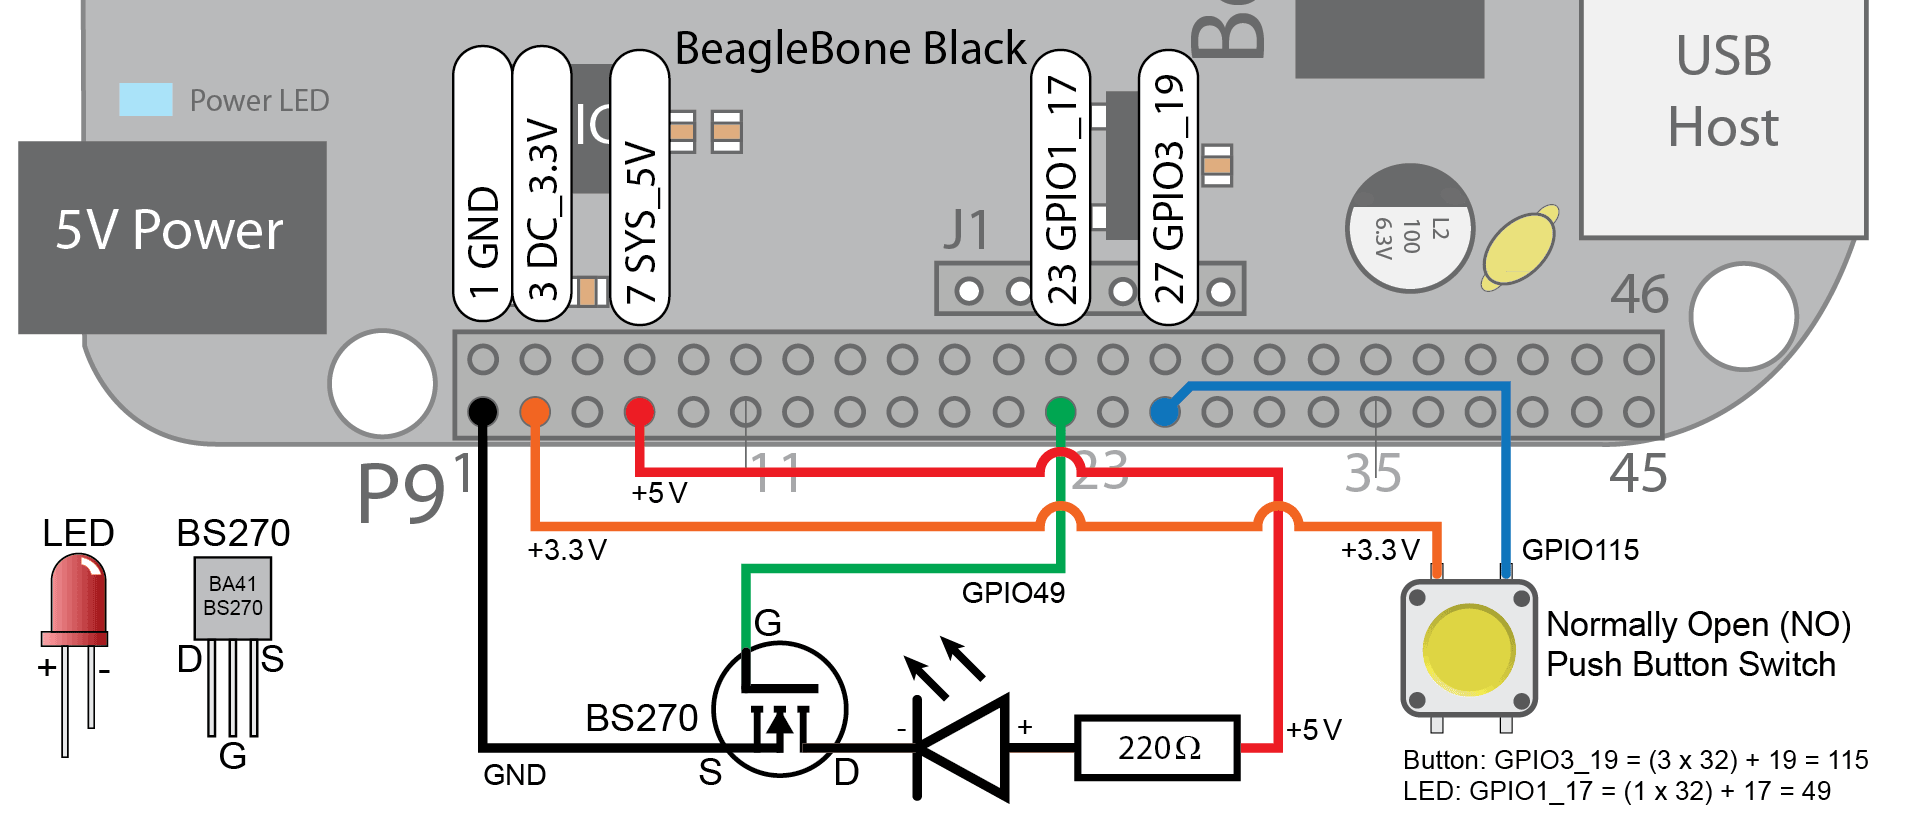
\includegraphics[width=0.875\textwidth]{Button-and-LED-large.png}
\end{center}
{\tiny \copyright \url[http]{derekmolloy.ie/kernel-gpio-programming-buttons-and-leds}}
\end{frame}

\section{\usp}
\begin{frame}{Vom \usp aus}{In Verzeichnis \cod{/sys/class/gpio}}
\begin{itemize}
 \item Output \cod{gpio49}
 \begin{itemize}
 \item \cod{cd gpio49}
 \item \cod{echo out > direction}
 \item \cod{echo 1 > value} \cod{echo 0 > value}
 \end{itemize}
 \item Input \cod{gpio115}
 \begin{itemize}
  \item entsprechend
 \end{itemize} 
\end{itemize}
\end{frame}

\begin{frame}{Aufgabe}{Skript}
 \begin{itemize}
  \item blink
  \item Polling
  \begin{itemize}
   \item read switch set led
  \end{itemize}
 \end{itemize}
\end{frame}

\section{LKM}
\subsection{linux/gpio.h}
\begin{frame}{Loadable Kernel Module (LKM)}{\cod{gpio-0.c}}
 \begin{itemize}
  \item eigenes Verzeichnis in  \cod{sys}: \cod{my-hw}
  \item einen File \cod{led} mit \cod{rw}:
  \begin{itemize}
   \item write: \cod{echo {\em x}> /sys/my-hw/led}
   \begin{description}[x=t$|$T]
    \item[x=1] set led
    \item[x=0] clear led
    \item[x=t$|$T] toggle led
   \end{description} 
   andere Werte von \cod{x} �ndern nichts
   \item read: \cod{cat /sys/my-hw/led}
   \begin{description}
    \item [1] led on
    \item [0] led off
   \end{description} 
  \end{itemize} 
 \end{itemize}
\end{frame}

\begin{frame}{Was Sie brauchen}{Pin 49 ist Output}
\begin{itemize}
 \item  \href{https://elixir.bootlin.com/linux/latest/source/include/linux/gpio.h\#L115}
             {\cod{gpio\_request}}
 \item  \href{https://elixir.bootlin.com/linux/latest/source/include/linux/gpio.h\#L131}
             {\cod{gpio\_free}}
 \item  \href{https://elixir.bootlin.com/linux/latest/source/include/linux/gpio.h\#L152}
             {\cod{gpio\_direction\_output}}
 \item \href{https://elixir.bootlin.com/linux/latest/source/include/linux/gpio.h\#L169} 
             {\cod{gpio\_set\_value}}            
\end{itemize}     
\end{frame}

\subsection{Direkt GPIO}
\begin{frame}{Loadable Kernel Module (LKM)}{\cod{gpio-1.c}}
\begin{itemize}
 \item Manual \cod{spruh73l.pdf} Abschnitt 25
 \item \cod{gpio.h} die einzelnen Register
 \item \href{https://elixir.bootlin.com/linux/latest/source/arch/alpha/include/asm/io.h\#L286}
            {\cod{ioremap}}
 \item \href{https://elixir.bootlin.com/linux/latest/source/arch/alpha/include/asm/io.h\#L306}
            {\cod{iounmap}}        
\end{itemize}
\end{frame}
\end{document}
